\documentclass[border=3pt]{standalone}
\usepackage{tikz}
\usepackage{amsmath}
\usepackage{amssymb}
\usepackage{ctex}
\usetikzlibrary{matrix, calc, positioning}
\usepackage{pgfplots}
\pgfplotsset{compat=1.18}

\begin{document}
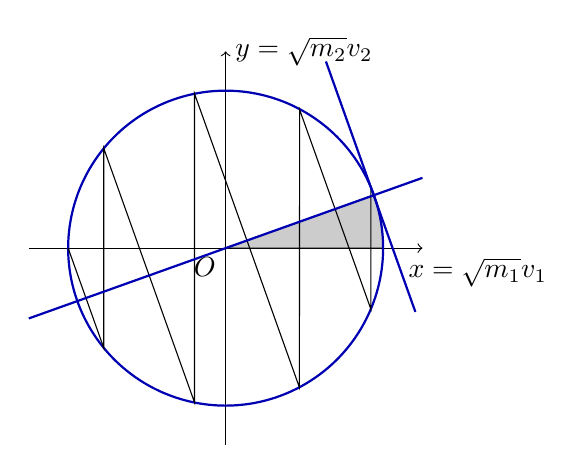
\begin{tikzpicture}
  \draw[->](-2.5,0)--(2.5,0)node[below,xshift=2em]{$x =
  \sqrt{m_{1}}v_{1} $};
  \draw[->](0,-2.5)--(0,2.5)node[right]{$y = \sqrt{m_{2}}v_{2} $};
  \node[below left]at(0,0){$O$};
  \draw[samples=1000, fill=gray!40]
  (0,0) --(0:2) arc(0:19.65382:2) -- cycle;
  \draw[domain=0:360,samples=1000, smooth, thick, blue!70!black]
  plot({2*cos(\x)},{2*sin(\x)});
  \draw (-2,0) --
  (-1.54751,-1.26697)--(-1.54751,1.26697)--(-0.39479,-1.96065)--(-0.39479,1.96065)--(0.93657,-1.76716)--(0.94,1.75755)--(1.84414,-0.77404)--(1.84414,0.77405)--(1.91726,0.56931);
  \draw[domain=1.274:2.41,samples=1000, smooth, thick, blue!70!black]
  plot({\x},{-2.8*(\x-1.84414)+0.77404});
  \draw[domain=-2.5:2.5,samples=1000, smooth, thick, blue!70!black]
  plot({\x},{0.3571428*(\x)});
\end{tikzpicture}
\end{document}
